\newcommand{\svcourse}{CST Part IA: Introduction to Probability}
\newcommand{\svnumber}{1}
\newcommand{\svvenue}{Churchill, Room TBD}
\newcommand{\svdate}{2022-05-14}
\newcommand{\svtime}{11:00}
\newcommand{\svuploadkey}{PO5ogKIM8KQA22FZS8IAf8gxA8XKi19jxIBVHIfFZ+3GCBXuNUXS9lVN6bNYjxM/}

\newcommand{\svrname}{Mr Matthew Ireland}
\newcommand{\jkfside}{twoside}
\newcommand{\jkfhanded}{right}

\newcommand{\studentname}{Harry Langford}
\newcommand{\studentemail}{hjel2@cam.ac.uk}


\documentclass[10pt,\jkfside,a4paper]{article}
\usepackage{tikz}

% DO NOT add \usepackage commands here.  Place any custom commands
% into your SV work files.  Anything in the template directory is
% likely to be overwritten!

\usepackage{fancyhdr}

\usepackage{lastpage}       % ``n of m'' page numbering
\usepackage{lscape}         % Makes landscape easier

\usepackage{verbatim}       % Verbatim blocks
\usepackage{epsfig}         % Embed encapsulated postscript
\usepackage{array}          % Array environment
\usepackage[nolinks]{qrcode}         % QR codes
\usepackage{enumitem}       % Required by Tom Johnson's exam question header

\usepackage{hhline}         % Horizontal lines in tables
\usepackage{siunitx}        % Correct spacing of units
\usepackage{amsmath}        % American Mathematical Society
\usepackage{amssymb}        % Maths symbols
\usepackage{amsthm}         % Theorems

\usepackage{ifthen}         % Conditional processing in tex

\usepackage[top=3cm,
            bottom=3cm,
            inner=2cm,
            outer=5cm]{geometry}

% PDF metadata + URL formatting
\usepackage[
            pdfauthor={\studentname},
            pdftitle={\svcourse, SV \svnumber},
            pdfsubject={},
            pdfkeywords={9d2547b00aba40b58fa0378774f72ee6},
            pdfproducer={},
            pdfcreator={},
            hidelinks]{hyperref}

\renewcommand{\headrulewidth}{0.4pt}
\renewcommand{\footrulewidth}{0.4pt}
\fancyheadoffset[LO,LE,RO,RE]{0pt}
\fancyfootoffset[LO,LE,RO,RE]{0pt}
\pagestyle{fancy}
\fancyhead{}
\fancyhead[LO,RE]{{\bfseries \studentname}\\\studentemail}
\fancyhead[RO,LE]{{\bfseries \svcourse, SV~\svnumber}\\\svdate\ \svtime, \svvenue}
\fancyfoot{}
\fancyfoot[LO,RE]{For: \svrname}
\fancyfoot[RO,LE]{\today\hspace{1cm}\thepage\ / \pageref{LastPage}}
\fancyfoot[C]{\qrcode[height=0.8cm]{\svuploadkey}}
\setlength{\headheight}{22.55pt}

\ifthenelse{\equal{\jkfside}{oneside}}{

 \ifthenelse{\equal{\jkfhanded}{left}}{
  % 1. Left-handed marker, one-sided printing or e-marking, use oneside and...
  \evensidemargin=\oddsidemargin
  \oddsidemargin=73pt
  \setlength{\marginparwidth}{111pt}
  \setlength{\marginparsep}{-\marginparsep}
  \addtolength{\marginparsep}{-\textwidth}
  \addtolength{\marginparsep}{-\marginparwidth}
 }{
  % 2. Right-handed marker, one-sided printing or e-marking, use oneside.
  \setlength{\marginparwidth}{111pt}
 }

}{
 % 3. Alternating margins, two-sided printing, use twoside.
}

\setlength{\parindent}{0em}
\addtolength{\parskip}{1ex}

% Exam question headings, labels and sensible layout (courtesy of Tom Johnson)
\setlist{parsep=\parskip, listparindent=\parindent}
\newcommand{\examhead}[3]{\section{#1 Paper #2 Question #3}}
\newenvironment{examquestion}[3]{
    \examhead{#1}{#2}{#3}\setlist[enumerate, 1]{label=(\alph*)}\setlist[enumerate, 2]{label=(\roman*)}
    \marginpar{\qrcode{https://www.cl.cam.ac.uk/teaching/exams/pastpapers/y#1p#2q#3.pdf}}
    \marginpar{\footnotesize \url{https://www.cl.cam.ac.uk/teaching/exams/pastpapers/y#1p#2q#3.pdf}}
}{}



\begin{document}

\begin{enumerate}

\item Describe a 5-stage pipeline suitable for executing the RISC-V ISA .

Here are the main parts of executing an instruction and a dependency
graph for the RISC-V ISA. As we can see, there are 5 stages which must be done
serially. Therefore the 5-stage pipeline will be Instruction Fetch;
Decode \& Operand Fetch; Execute \& Branch; Memory Access and Writeback.

\begin{center}
\begin{tikzpicture}
\node (IF) at (0, 0) {Instruction Fetch};
\node (D) at (3, 0.5) {Decode};
\node (OF) at (3, -0.5) {Operand Fetch};
\node (E) at (6, 0.5) {Execute};
\node (B) at (6, -0.5) {Branch};
\node (MA) at (9, 0) {Memory Access};
\node (W) at (12, 0) {Writeback};
\draw [-stealth] (IF) -- (D);
\draw [-stealth] (IF) -- (OF);
\draw [-stealth] (D) -- (E);
\draw [-stealth] (OF) -- (E);
\draw [-stealth] (D) -- (B);
\draw [-stealth] (OF) -- (B);
\draw [-stealth] (E) -- (MA);
\draw [-stealth] (B) -- (W);
\draw [-stealth] (MA) -- (W);
\end{tikzpicture}
\end{center}

\begin{itemize}

\item Instruction Fetch

Load the value addressed by the program counter into the ``instruction
register'' and increment the program counter.

\item Decode \& Operand Fetch

Decode the instruction to determine what operation we are performing. In
this stage we also determine which bits are immediates and determine the
value of any immediates. In parallel we can load two operands (rs1 and rs2)
from the registers. Although some instructions only require one operand, it
is far faster to load both and discard one if it's not needed. The RISC-V is
designed to make this particularly easy -- all source registers are stored
in the same place.

\item Execute \& Branch

Perform an arithmetic or logical operation and if necessary update the
program counter. Although branch is writing back to a register, it makes
more sense to write to the program counter as soon as we know it has to be
written to. This will reduce the branch-taken penalty.

\item Memory Access (MA)

Read from or store to memory if required. Most instructions will not need to
access memory.

\item Writeback (W)

We store the result of the instruction in the destination register if there
is any result to be stored.

\end{itemize}

\item What is the significance of some registers being preserved in some
circumstances and others not?

The reason that some registers are preserved is that the calling convention
denotes some registers should be nonvolatile in order to retain a consistent
ABI (Application Binary Interface). While others are volatile and have no such
constraints.

If a function preserves a register, then the value of that register after
the function call is the same as the value at the start of the function call.

A Calling convention defines which registers should be preserved. It
defines a set of registers as ``nonvolatile'' -- meaning the caller should
expect these registers to contain the same value at the end of the function
call as at the beginning. Failure to preserve these registers will cause
the caller to lose data. This provides a consistent interface between
functions and allows good integration.

Other registers are ``volatile'', meaning the callee can overwrite these
freely.

\item What control hazards apply to your pipeline and how could they be
resolved?

When branching, we know the updated value of the PC and update it at the end
of the execute stage. However, the two next instructions could have fetched
from the wrong address. The simplest solution is therefore to flush the next
two instructions. Note that commits are only made after the execute stage --
writing to the PC in execute, storing to memory in memory access or writing
to registers in write-back. Therefore the two instructions we would cancel
will not have made any commits and so we do not have to ``undo'' them.

A more efficient (and complicated) approach involves branch prediction. We
``guess'' which instructions will be executed next and execute those, only
flushing the pipeline if we are incorrect. This method requires much more
hardware but can increase performance significantly.

Branch prediction can be split into two slightly different cases,
conditional branches and unconditional branches.

Unconditional branches are the simpler case. The processor reads ahead
checking for an unconditional branch and updates the PC immediately after
the instruction unconditional branch is issued. If the unconditional branch
jumps by an immediate such as JAL, then we can update the program counter on
issuing the instruction. If the unconditional branch branches by the value
in a register (such as JALR), then we can ``guess'' what the value of that
register will be and speculatively execute the next instructions. Generally
this guess will be that the value of the register has not changed -- it's not
common for functions to update their own return addresses. If this
speculation was incorrect then we flush the 2 next instructions after
executing successfully and reset the program counter.

Conditional branches are similar to JALR -- the location of the following
instruction jump is not known until after the instruction is executed. The
most efficient solution is to speculate about whether the branch will be
taken or not. The complexity of branch predictors ranges from ``backwards
branches (loops) are usually taken and forward branches aren't'' to machine
learning models built into hardware.

If we speculatively executed correctly, then we have no pipeline bubbles and
increase our processors performance significantly. If we guess incorrectly
then we lose nothing. Modern branch predictors can have 99\% accuracy
meaning that the expected cost of a branch instruction decreases from 3 cycles
to 0.03 cycles.

There is lots of literature on branch prediction -- compiler optimisations
and implementation details.

\item What data hazards apply to your pipeline and how could they be resolved?

There are three data hazards in this pipeline. Two can be resolved without
any inefficiency, while resolving the third is more complicated and will
decrease performance.

\begin{itemize}

\item Execute, Execute

If we execute an instruction which will change the result in a register $r_i$
and the next instruction has $r_i$ as an operand; then the next instruction
will have the outdated version of $r_i$.

We can resolve this by adding a feed-forward path from the output of execute
to the input of execute. This will update the value of any registers which
have been modified and are used in the next instruction. Hence providing
the next instruction with the updated value for $r_i$ with no stalls.

\item Store, Decode

If we update a register at the same time that register is being fetched in
the Decode stage, the value fetched from that register will be outdated -- a
data hazard. This can be resolved by storing to registers in the first half
of the clock cycle and fetching from them in the second half. Therefore
Decode will fetch the correct value.

\item Memory-Access, Decode, Execute,

Memory accesses take time. Evven an L1 cache hit takes $\sim 3$ clock cycles.
Higher level caches take tens of cycles and DRAM takes hundreds. In the
worst-case, a memory access could cause a page fault, requiring hundreds of
thousands of cycles to load the memory in from the hard disk. Between the
time that a memory access is started and returns, we cannot execute any
instructions which depend on the fetched instruction.

The ``solution'' is to execute only instructions which do not depend the
result of the memory access until the memory access returns. There are four
ways to do this.

The simplest solution is to flush the pipeline after the memory access and
issue NOPs until the memory access returns. This could cause the processor
to frequently stall, dramatically reducing performance and making any
computer almost unusable. This may be a suitable approach on very simple
processors such as in embedded systems with very small memories. However,
this is not a viable solution in the general case.

In Dynamic Scheduling, the hardware reorders the order in which instructions
are issued while preserving data flow and exception behaviour. If we reorder
the instructions to maximise the amount of time after a memory access before
the fetched value is needed, then we can give the instruction time to complete
before the processor stalls, allowing dozens or even hundreds of extra cycles
before the value is needed. This can virtually eliminate the performance hit
from cache hits. However, on cache misses or page faults Dynamic Scheduling
will have a small impact. Additionally, Dynamic Scheduling cannot
\textit{always} reorder well; meaning sometimes even cache hits will cause
stalls.

Multithreading allows the processor to execute code without any data
dependencies. For a single-issue processor\footnote{talking about data
dependency resolution in superscalars, VLIW or EPIC would be dramatic
overkill -- this would add synchronous multithreading} such as we are
talking about, there are two types of multithreading: fine-grained and
course-grained multithreading. In fine-grained multithreading, consecutive
instructions are issued by different threads -- if one stalls then the other
will issue on consecutive cycles until the memory access returns. The second
type of multithreading is coarse-grained multithreading; when the first
thread stalls the others will start issuing instructions. Implementing
either type of multithreading will require multiple sets of registers -- one
per thread.

The final ``solution'' is to context switch. If a process can truly execute
nothing for hundreds of thousands or millions of cycles, then yielding may
be more efficient. For example if a process with a single thread attempts to
read from memory a value which all subsequent instructions depend on and causes
a page fault then it may yield and allow another process to execute while
the memory access takes place. This decision should be based on an estimate
of how long until the memory access will return versus how long it will take
to context switch.

\end{itemize}

\item What restrictions on memory accesses are imposed by your ISA?

% TODO: this answer feels a bit weak

I will interpret ``your ISA'' as the ISA the pipeline in previous sections
uses (RISC-V) rather than the ISA my computer uses (x86-64).

The pipeline in previous stages is using the RISC-V ISA .

RISC-V imposes the following restrictions on memory accesses:

\begin{itemize}

\item RISC-V is a load-store architecture. This means that only load and
store instructions can access memory; arithmetic instructions can only operate
on CPU registers. This means we cannot update a single-use value in memory
without first loading it into a register -- potentially displacing the
value stored in that register, meaning we have to reloading the original value
afterwards. For example if we wish to increment all values of a
contiguous array (ignoring RISC-V vector extensions); we have to load all
values into registers one-by-one and then store them back rather than using
a single instruction to modify values in memory.

\item RISC-V has no instruction which accesses memory addressed by the sum
of two registers and an immediate. This is a common operation in
object-oriented languages which is provided by both ARM and x86. This omission
means RISC-V is less efficient for object-oriented languages.

\item The ISA will define a maximum pointer size. This limits the size of
memory which the CPU can access. For example if we use RV32I, then we
cannot access more than 4GB of memory.

\end{itemize}

\item How does the i386 differ from RISC-V in goals and implementation

\begin{itemize}

\item i386 is a family of processors while RISC-V is an ISA .

The primary difference between the two is that i386 is a physical processor
on which code can be run, while RISC-V is a list of instructions which a
processor could implement.

\item i386 is proprietary

RISC-V was designed to be an open source ISA -- this means that anyone can
use it and build a processor using RISC-V . i386 was designed by Intel to be
built and sold by Intel; it is therefore proprietary.

\item i386 was designed to be backwards compatible

i386 was designed such that it would be able to run all previous x86 code --
both for previous 32-bit architectures and 16-bit architectures. Conversely,
RISC-V was a ``fresh-start'' without any backwards compatibility
requirements -- although many features were inherited from MIPS .

\item i386 ran on a CISC instruction set while RISC-V uses a RISC
instruction set.

i386 ran on the x86-32 instruction set. This is the 32-bit version of x86.
x86-32 was built with two optimisations in mind, ease of programming for
assembly-writers and optimising machine code size.

Conversely, RISC-V is designed to make the common case fast. It is designed
to have a smaller set of instructions which are easy to implement in
hardware and can allow the processor to run at a higher clock frequency.

\item x86-32 was designed for assembly writers

x86-32 was designed with the expectation that people would be routinely
writing assembly in it. Many x86-32 instructions are very specific and
obscure, but help bridge the semantic gap between high-level programs and
machine code.

RISC-V was designed to be a target for compilers with the expectation that
people would almost never directly write assembly. This means many RISC
instructions are simple but allow for good compiler optimisation. As a
result programming in RISC-V requires far more instructions than the
equivalent program in x86-32.

\item x86-32 has variable length instructions

x86-32 instructions are designed such that the most common instructions are
short and the least common instructions are very long. The result is that
x86-32 code is compressed almost to the entropy limit with instruction sizes
varying between 1 and 15 bytes. However, this makes decoding very
complicated. Determining where an instruction ends is difficult and we
cannot fetch from registers until we have done so. This serialises the
decoding process.

RISC-V has constant-length instructions. Each instruction is 4 bytes (in
both 32 and 64-bit systems) and the source and destination registers (if
applicable) are all stored in the same place. Therefore, decoding is simple
-- fetch the next 4 bytes and load from the registers specified at bits
[6:11] and [19:24]. Therefore different parts of decoding can be done in
parallel and this greatly speeds up execution.

\item RISC-V processors can have much higher clock frequencies

RISC-V has such simple instructions that processors can be clocked far
faster than those implementing x86 such as i386. The difference is
incomparable, however as i386 was designed in the mid 1980s and therefore
the hardware available was much lower quality.

For example common RISC-V processors can be clocked at 5GHz, while the
fastest i386 processor only had a clock speed of 40MHz.

\item i386 was built using 1980s ideas and technology

This means that i386 had very few additional features. For example it did
was not a superscalar processor, had no vector extensions and did not support
either dynamic execution or speculative execution. Instructions were
executed only if they were issued and they were executed in the order in
which they occurred in the code. An example of the technology available in
the 1980s is that the i386 cache used (the much slower) DRAM rather than SRAM.

RISC-V was designed with the intent of being run on all types of processors
and therefore has support for every modern feature and has space left for
many future ideas. RISC-V can have vector extensions, can be executed
out-of-order (dynamic scheduling) and is amenable to speculative execution.

\item i386 had specialised registers

x86-32 requires specialised registers, with many instructions performing very
specialised operations on single registers. Therefore i386 processors have
specialised instructions.

RISC-V instructions are orthogonal -- meaning that any instruction can be
applied with any register as argument (with the exception of the
destination register being x0) -- registers x1--x31 are general purpose.

\item i386 uses 32-bit addresses

The i386 family of processors used 32-bit addresses, RISC-V is designed to
support a range of address sizes. 32 and 64 bit are both supported and there
is work to standardise RV128I which would support 128 bit instructions.

\item x86-32 is monolithic

x86-32 was designed to be implemented in full by powerful microprocessors.
This means there is no ``minimal subset'' of x86-32 which could be
implemented. Implementing x86-32 requires implementing thousands of
instructions. This makes it very unfriendly for researchers to use.

Conversely, RISC-V was designed to be implementable by many different types
of projects and is therefore segmented into modules. A minimal
implementation of RISC-V requires only 50 instructions and other sets of
instructions can be added as required. There is also a small set of RISC-V
which is purposefully designed for use on tiny embedded systems (RV32E) and
requires only 16 registers.

\item x86-32 is complete

Many processors of all complexities have been implemented using x86-32,
therefore the instruction set is (largely) bug-free and is very well
specified. RISC-V is a very new ISA and is largely incomplete -- the basic
instructions are well-specified however, more advanced privileged
instructions, vector extensions and more are not well-specified.

\end{itemize}

\end{enumerate}

\end{document}
